\newpage

\section{Inertial Measurement Unit - Accelerometer, Rate Gyro, Magnetometer}

\subsection{Parts List}

\begin{enumerate}[itemsep=-5pt]
\item Laptop
\item CPX/CPB 
\item USB Cable
\item \href{https://www.adafruit.com/product/4485}{LSM6DS33+LIS3MDL} (Not included in kit. Note that other Inertial Measurement or "DOF" Sensors will work for this lab you will just have to change the code to accommodate the change in hardware)
\item Alligator Clips (x4)
\item Bread Board
\item Soldering iron
\end{enumerate}

\subsection{Learning Objectives}
\begin{enumerate}[itemsep=-5pt]
\item See and understand the concept of soldering
\item Understand the I2C protocol at a high level
\item Learn the components of an IMU (Accelerometer, Rate Gyro, Magnetometer)
\item Read IMU data and plot
\end{enumerate}

\subsection{Getting Started}

In this lab we’re going to use this an external sensor to measure angular velocity and the magnetic field of the surrounding environment.
\begin{figure}[H]
  \begin{center}
    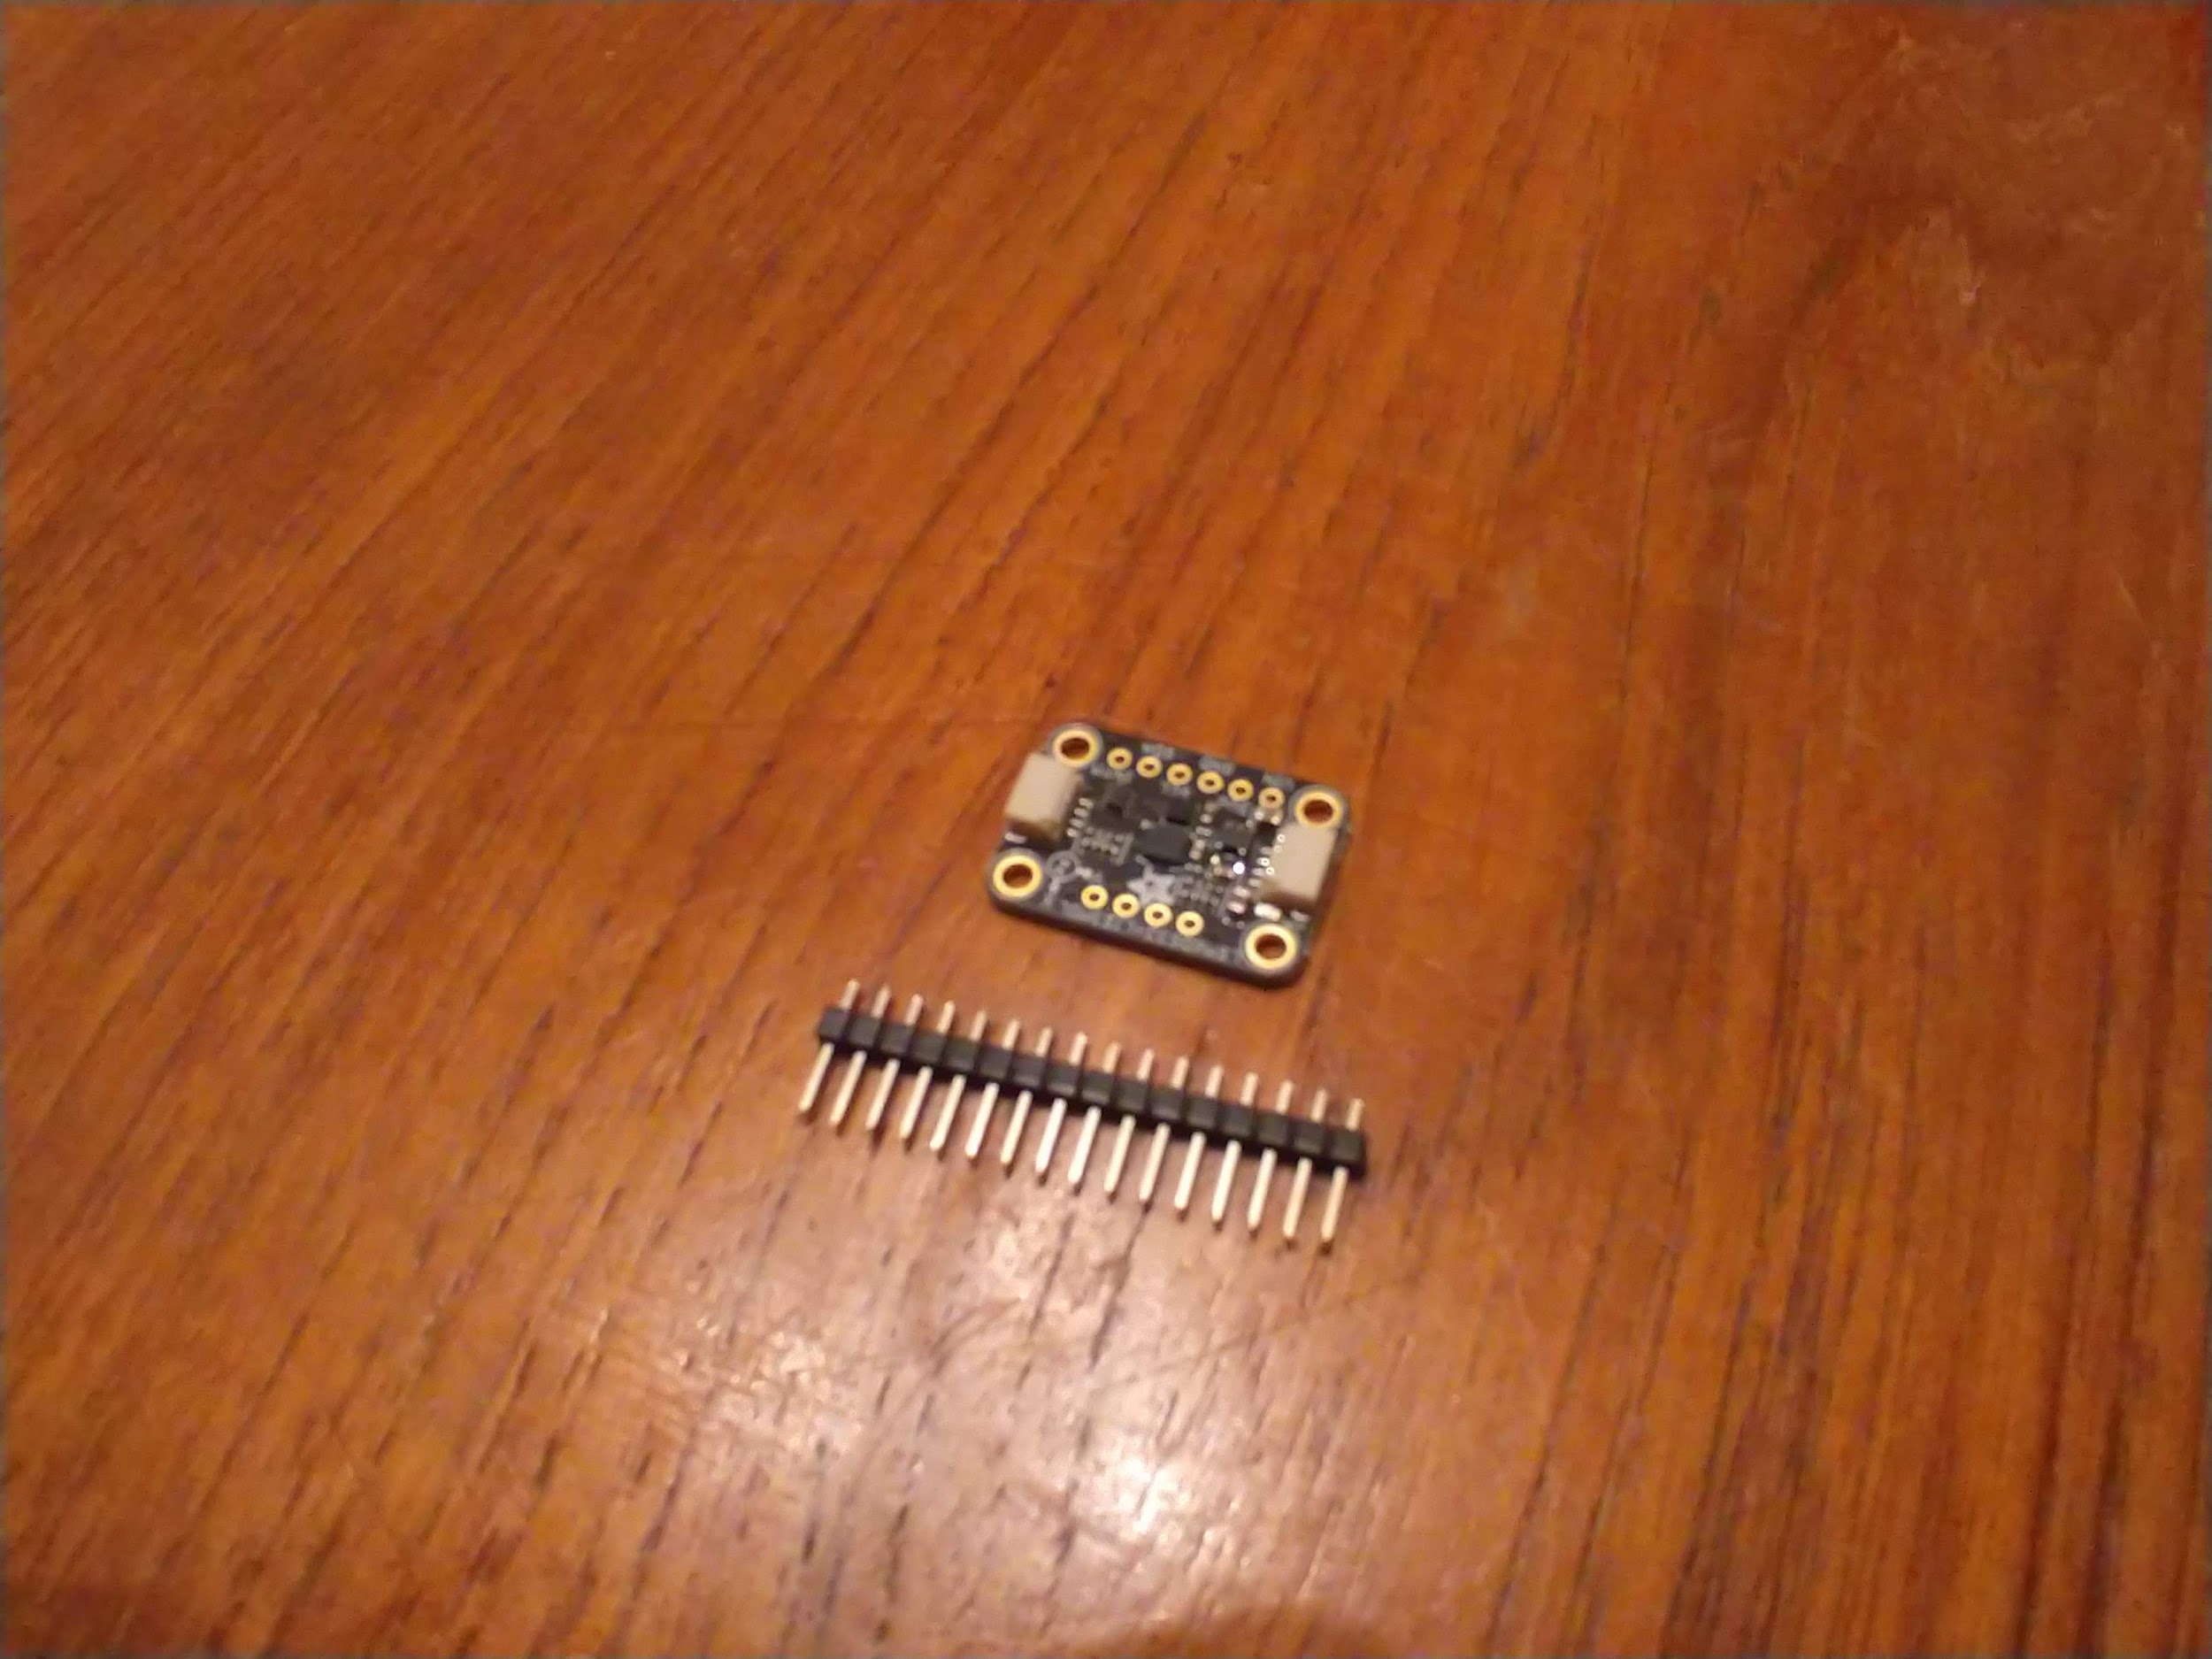
\includegraphics[width=\textwidth]{Figures/imu.jpeg}
  \end{center}
\end{figure}
The sensor above is the \href{https://www.adafruit.com/product/4485}{LSM6DS33+LIS3MDL}. You basically have 2 separate microchips in one. The first (LSM6DS33) is a 3-axis accelerometer and 3-axis rate gyro. The first measures acceleration and the second measures angular velocity. The LIS3MDL is a 3-axis magnetometer which measures magnetic fields. The three of these sensors put together (accelerometer, rate gyro, magnetometer) is called an IMU (Inertial Measurement Unit). It's actually possible to measure roll and pitch of an airplane and heading using the magnetometer. Combining the angular velocity of the rate gyro can create a complete attitude estimation algorithm for spacecraft. This sensor does not come standard in the current iteration of the kit. You can purchase one on Adafruit for only \$10 at the time of this writing. The interesting thing about this device is that you can actually purchase the LSM6DS33 and LIS3MDL separately but this breakout board has both chips on board. The goal of this lab is not necessarily to use this specific sensor but to understand IMUs and I2C protocol. Most if not all breakout boards on the Adafruit website use I2C communication. You'll know if the breakout board uses I2C if you find SDA/SCL pins on the board. It will also say it in the quick description of the sensor.
\begin{figure}[H]
  \begin{center}
    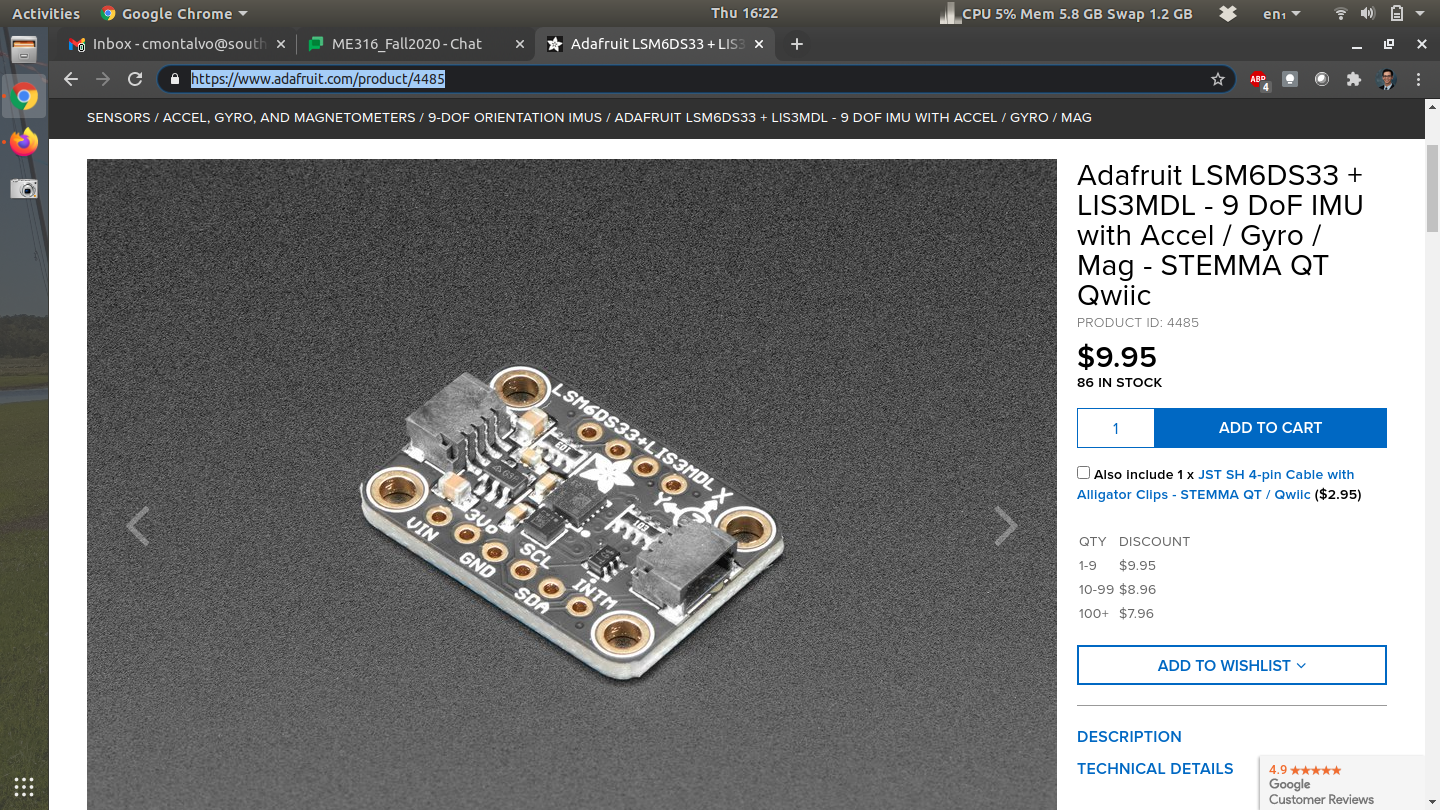
\includegraphics[width=\textwidth]{Figures/imu2.png}
  \end{center}
\end{figure}
When you open the packaging of this breakout board you’ll notice that the header pins are missing. First you’ll need to cut a row of 4 and 6 for the top and bottom side of the board and solder the header pins to sensor. If you’re taking my class you can stop by my lab one day and I’ll solder this for you or teach everyone about soldering during a lecture session of class. If you are taking this class elsewhere you have two options: try and find someone who can solder this real quick (only takes about 5 minutes) or buy your own soldering iron and try to solder yourself. Once the device is soldered you can "plug" it into a breadboard. Then, using 4 alligator clips you need VOUT (5V) to run to (VIN), GND to GND and then SDA to SDA and SCL to SCL.
\begin{figure}[H]
  \begin{center}
    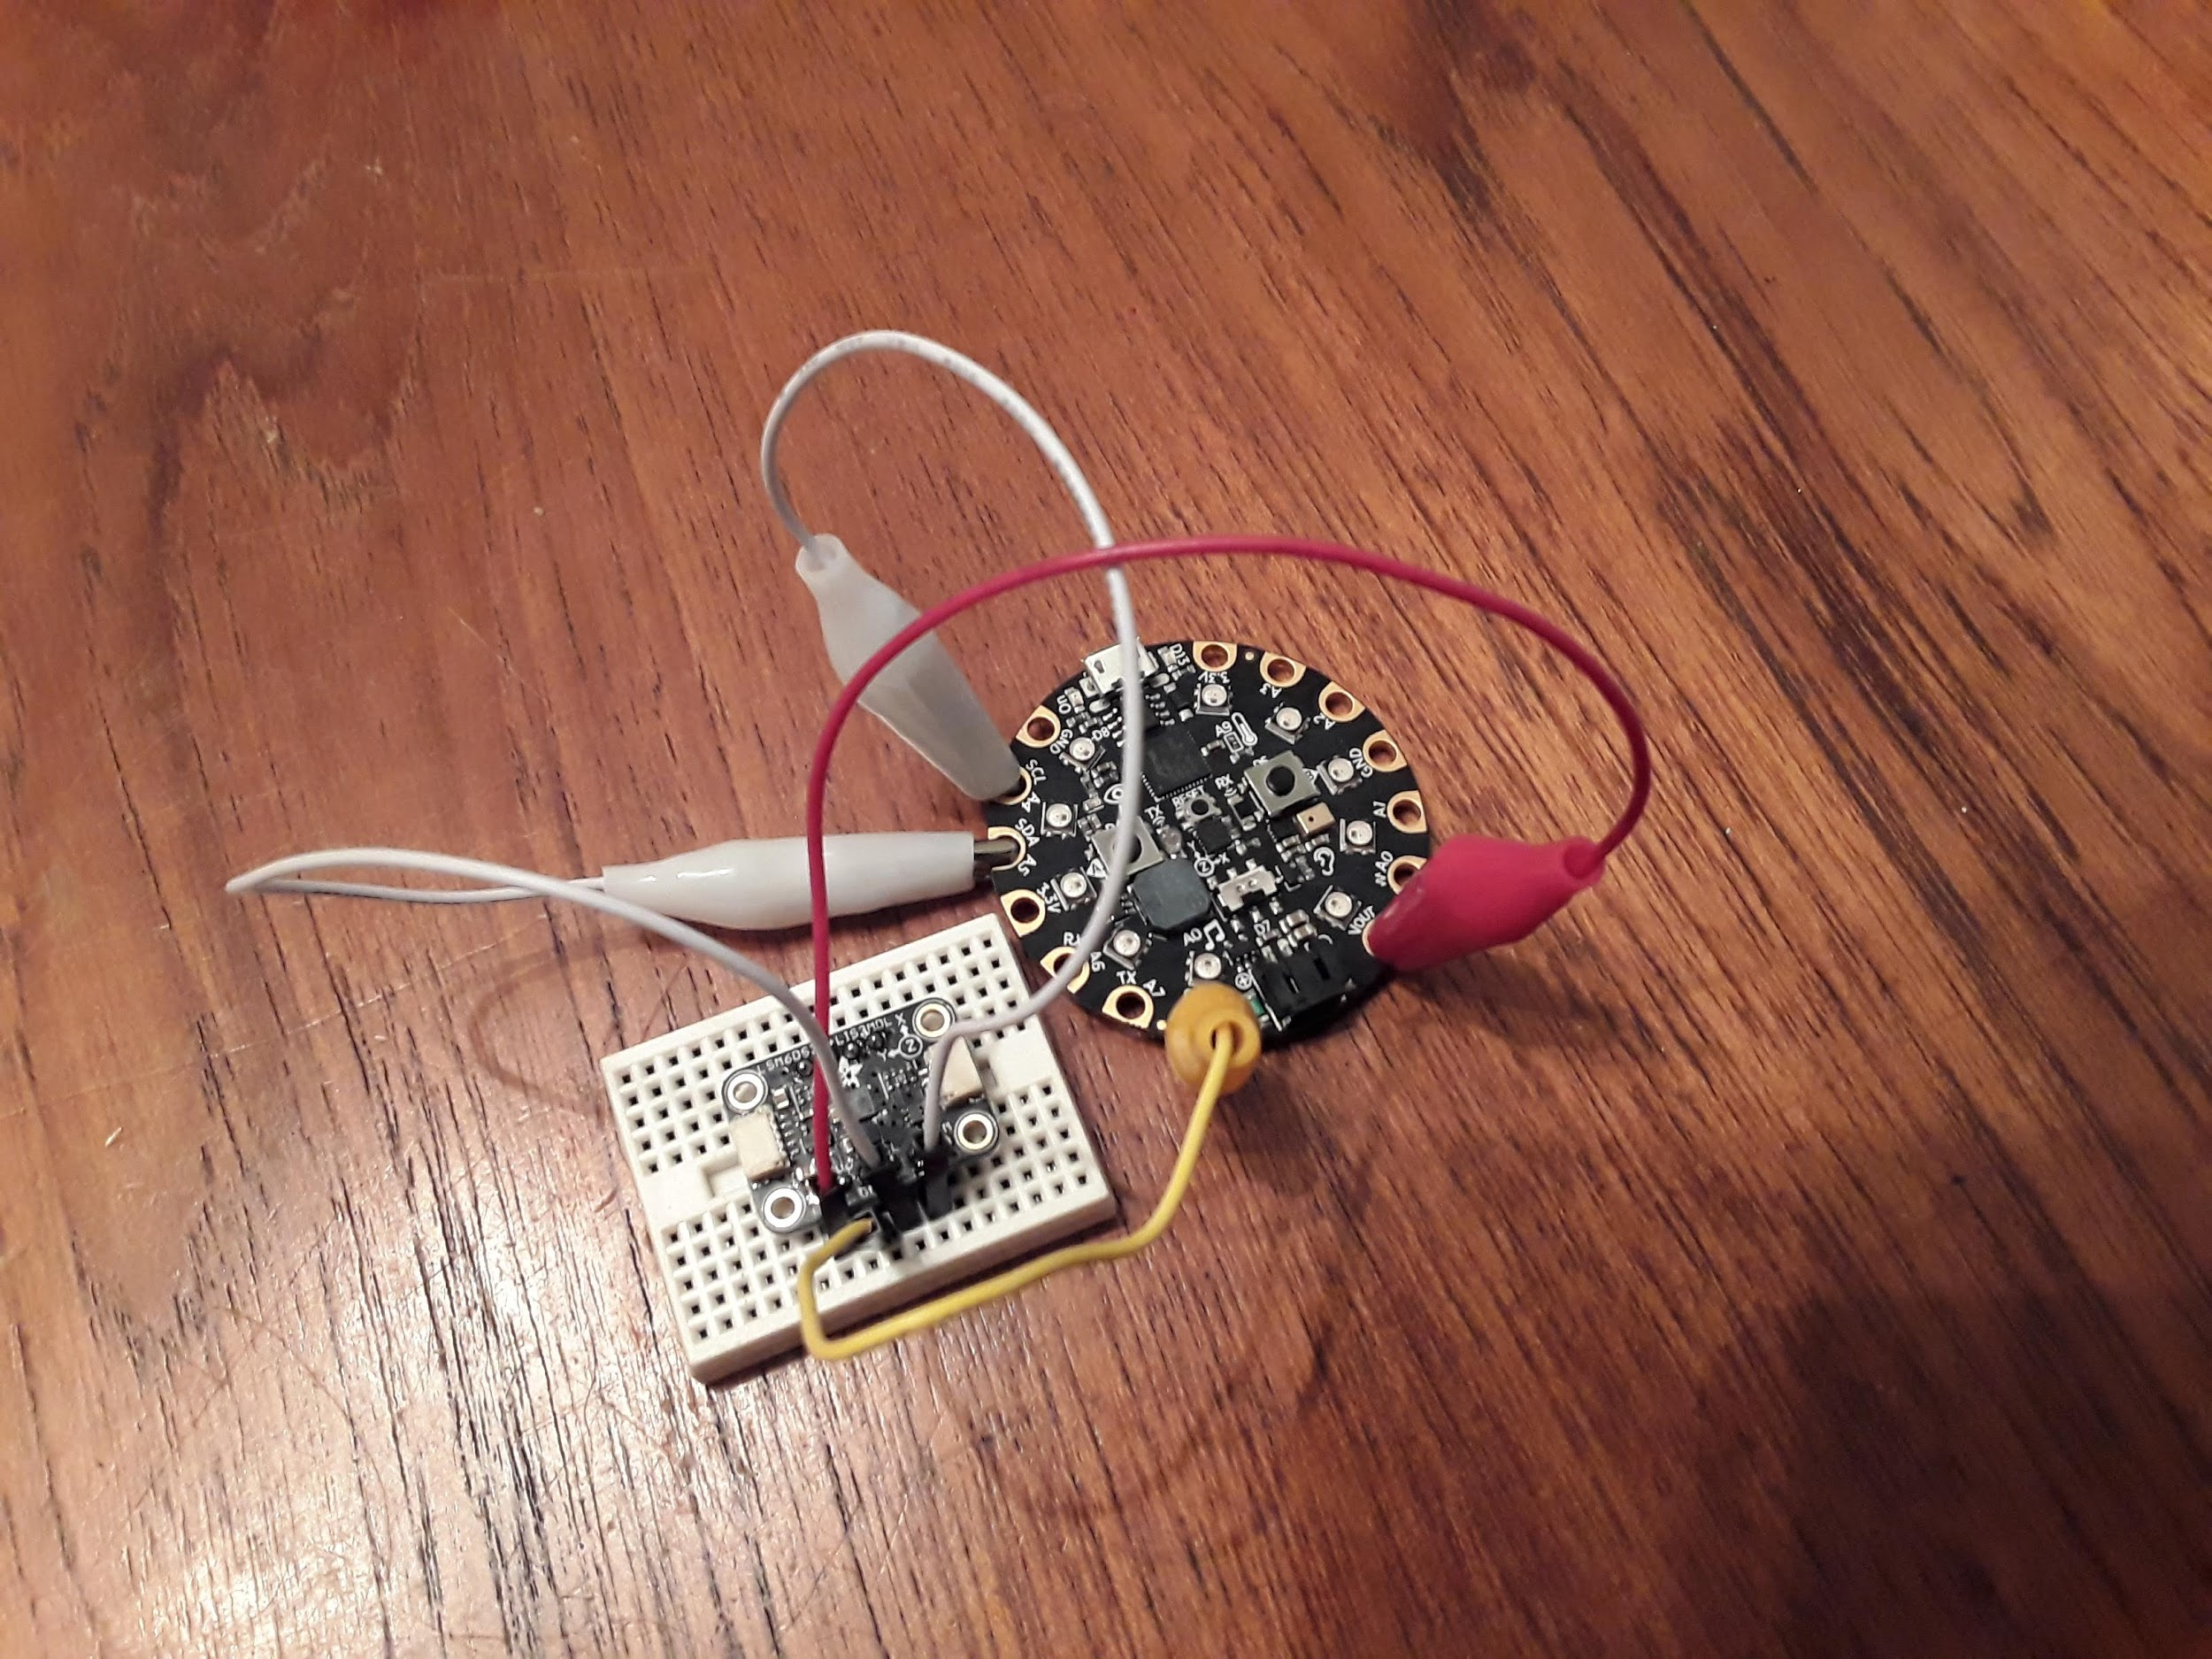
\includegraphics[width=\textwidth]{Figures/imu_circuit.jpeg}
  \end{center}
\end{figure}
Believe it or not the photo above was actually wired wrong. I had SDA to SCL and SCL to SDA. You need to make sure you have the proper wires going to the correct pins or it won’t work. SDA and SCL are 2 pins for something called I2C (pronounced I squared C) where I is I as in "I am a billy goat" or "I like to code". I2C is beyond the scope of this project but just know it’s a type of serial communication that uses hexadecimal addresses.

Once you have the circuit wired and soldered it’s time to work on software. First want to make sure you have your \href{https://circuitpython.org/downloads}{Circuit Python UF2} up to date. In this example I’m using the 6.X version. Once I updated my UF2 I also updated my \href{https://circuitpython.org/libraries}{Circuit Python Libraries}. The Circuit Python Libraries download as a zip file. You need to unzip the folder and go into the lib folder and grab the following python modules.
\begin{enumerate}[itemsep=-5pt]
\item adafruit\_bus\_device
\item adafruit\_register
\item lis3mdl
\item lsm6ds33
\end{enumerate}
There will be folders for some and just floating .mpy files for others which are python modules that you can import just like time, board and busio as we’ve done in the past. Put those files into your lib folder on your CIRCUITPY drive. If the lib folder doesn’t exist you just need to make one. Once you have the necessary modules you can run some example code. The Adafruit Learn page has a \href{https://learn.adafruit.com/lsm6ds33-6-dof-imu=accelerometer-gyro/python-circuitpython}{tutorial for the LSM6DS33}. The problem with the tutorial is that it seems like it was written for the Raspberry or some other microcontroller. As such I had to find some example code on \href{https://github.com/adafruit/Adafruit_CircuitPython_LSM6DS/blob/master/examples/lsm6ds_lsm6ds33_simpletest.py}{Adafruit's Github}. After following both tutorials I was able to make my own script and upload it to my \href{https://github.com/cmontalvo251/Microcontrollers/blob/master/Circuit_Playground/CircuitPython/Accelerometer/external_lis3mdl_lsm6dss.py}{Github}.
\begin{figure}[H]
  \begin{center}
    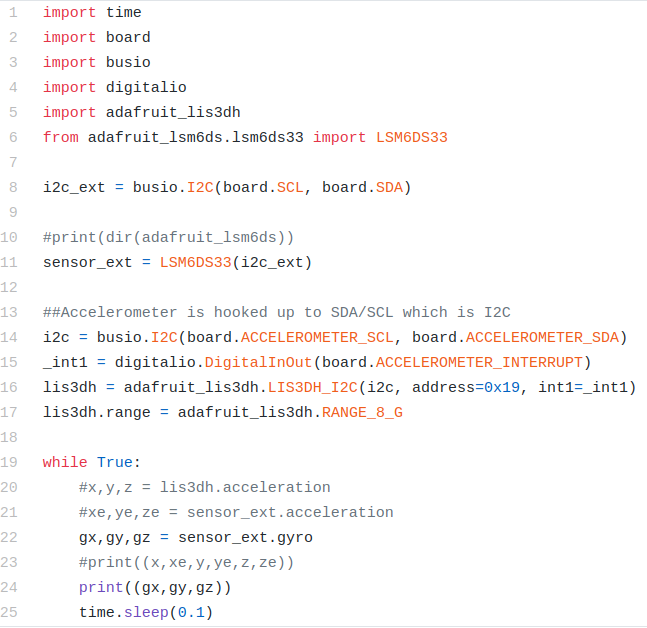
\includegraphics[width=0.8\textwidth]{Figures/imu_code.png}
  \end{center}
\end{figure}
In the code above lines 1-6 import all the modules with line 5 importing the accelerometer on board the CPX and line 6 importing the external sensor wired up to SDA and SCL. Line 8 creates an I2C object using the SDA and SCL pins from the alligator clips and line 11 creates the sensor object. I also include lines 14-17 to include the onboard accelerometer. Notice I can access both sensors no problem. In the while loop line 20 checks the accelerometer on the CPX, line 21 checks the accelerometer on the breakout board and line 22 checks the angular velocity on the breakout board. Lines 23 and 24 print to serial and output to the plotter. Note that some lines are commented out because I wanted to try one thing at a time. With both accelerometers printing to the Plotter I could move the CPX and the breakout board in unison and get the following output.
\begin{figure}[H]
  \begin{center}
    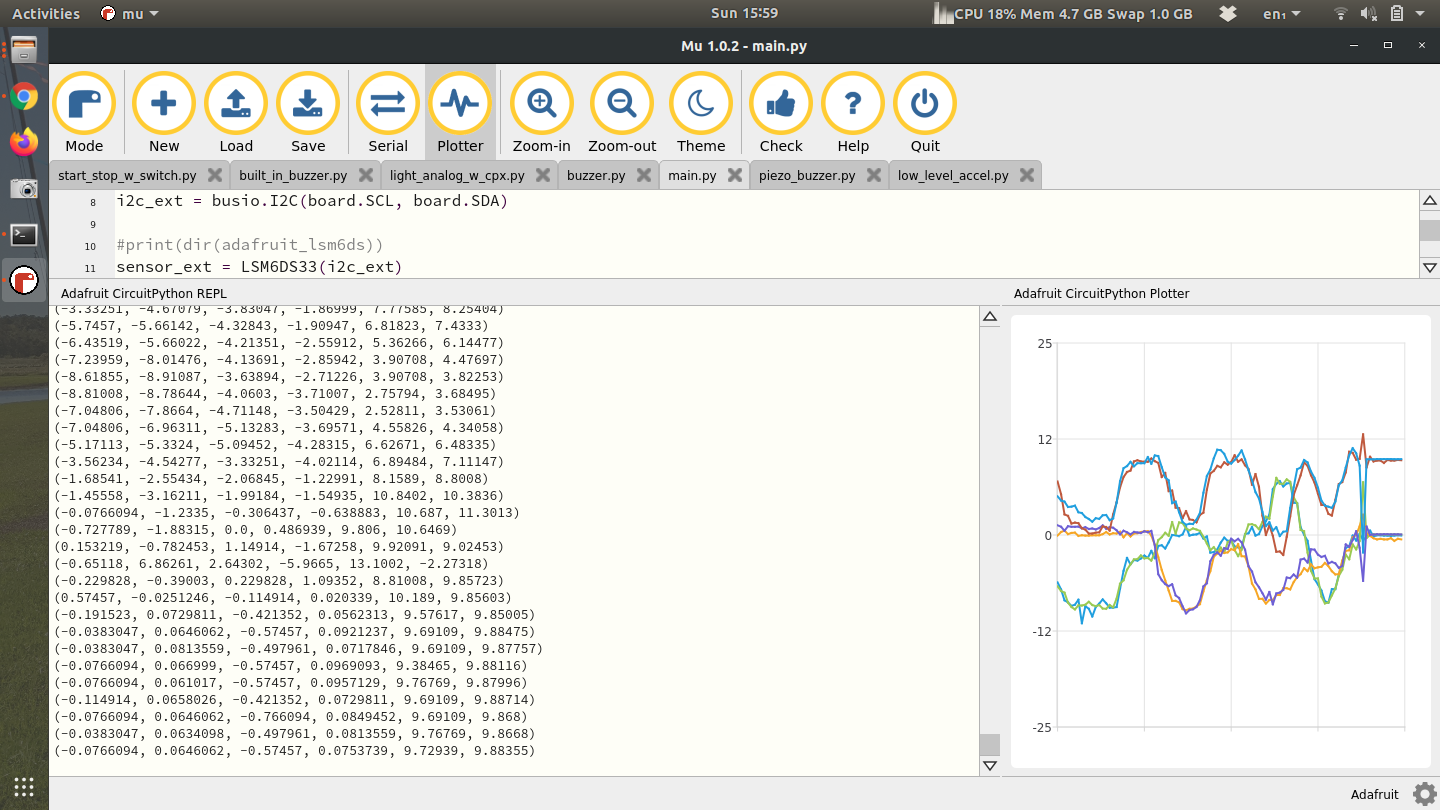
\includegraphics[width=\textwidth]{Figures/imu_mu.png}
  \end{center}
\end{figure}
Notice that there are 6 numbers printed and 6 lines on the plotter. Both the CPX and the breakout board have little XYZ cartesian coordinate systems. I had to line them up properly before I started moving them. My suggestion would be for you to get some hot glue or 3M tape and place both breakout board and CPX on some sort of hard material like plywood, masonite, or even a cutting board. Anything to keep everything together.

Once you’ve done this, try uncommenting the line of code that prints the angular velocity. When I do that and move the breakout board around I can measure the angular velocity of each axis. The units are in radians per second but it’s pretty obvious just from the magnitude of the graph.
\begin{figure}[H]
  \begin{center}
    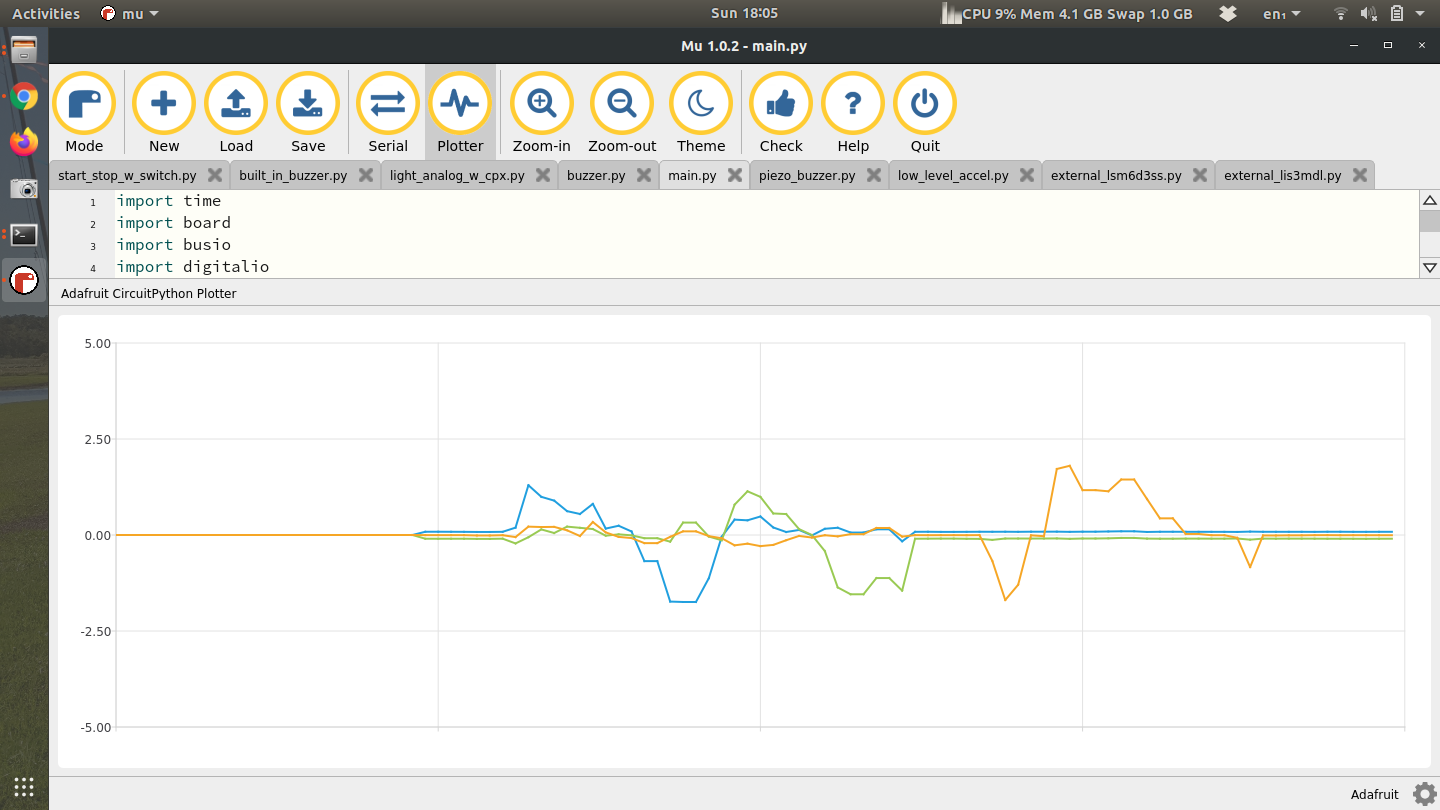
\includegraphics[width=\textwidth]{Figures/imu_mag.png}
  \end{center}
\end{figure}
The final part is to get the LIS3MDL (magnetometer) to work. The starting point for me was the \href{https://learn.adafruit.com/lis3mdl-triple-axis-magnetometer/python-circuitpython}{Adafruit Learn page}, along with the simple example from \href{https://github.com/adafruit/Adafruit_CircuitPython_LIS3MDL/blob/master/examples/lis3mdl_simpletest.py}{Adafruit's Github}. After that I was able to create \href{https://github.com/cmontalvo251/Microcontrollers/blob/master/Circuit_Playground/CircuitPython/Accelerometer/external_lis3mdl.py}{my own code}. The only difference in your code is that the address will be 0x1c instead of 0x1e.
\begin{figure}[H]
  \begin{center}
    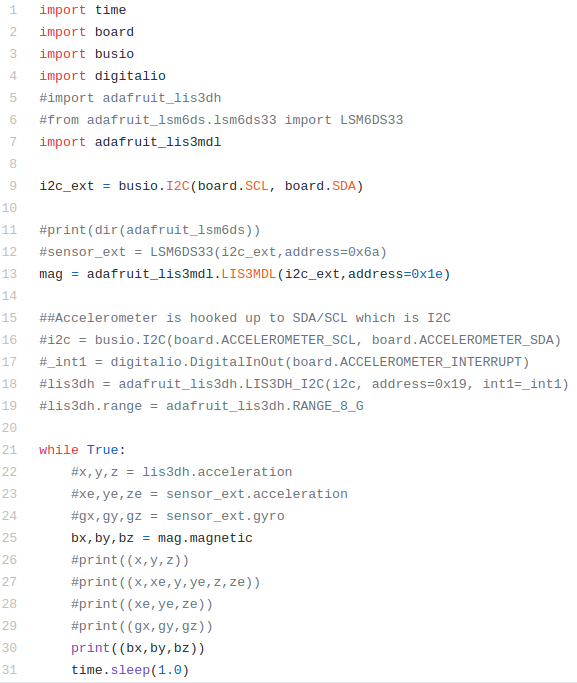
\includegraphics[width=0.8\textwidth]{Figures/imu_code_mag.png}
  \end{center}
\end{figure}
The code is almost identical to the code before except all the LIS3DH and LSM6DS33 code is commented out. Instead I have code to grab the magnetometer (LIS3MDL) at address 0x1E. Line 25 then calls the magnetometer and prints it. Note that the accelerometer can be used to obtain pitch and roll angles and the magnetometer can be used to obtain the yaw angle. This is done via trigonometry and is shown in the equations below. 
\begin{equation}
\theta = -sin^{-1}(\bar{a}_x)
\end{equation}
\begin{equation}
\phi = tan^{-1}\left(\frac{\bar{a}_y}{\bar{a}_z}\right)
\end{equation}
\begin{equation}
\psi = tan^{-1}\left(\frac{\bar{\beta}_z s_{\phi} - \bar{\beta}_y c_{\phi}}{\bar{\beta}_x c_{\phi} + \bar{\beta}_y s_{\theta}s_{\phi} + \bar{\beta}_z c_{\phi}s_{\theta}}\right)
\end{equation}
In the equations above $\beta$ is the magnetic field along all 3 axes and $a$ is the accelerations along all 3 axes. Shorthand is used for $cos(\eta)=c_{\eta}$ and $sin(\eta)=s_{\eta}$. The $\bar{\eta}$ notation is used to indicate a normalization of the vector. That is $\bar{\eta} = \eta/||\eta||$ where $||\eta||$ is the norm of a 3 dimensional vector $||\eta||=\sqrt{\eta_x^2+\eta_y^2+\eta_z^2}$. The derivation for these angles from accelerometers and magnetometers is quite involved and requires the knowledge of rotation matrices. That derivation is in another textbook called \href{https://github.com/cmontalvo251/LaTeX/tree/master/Aerospace_Mechanics}{Aerospace Mechanics}.

\subsection{Assignment}

For this assignment you are to wire up the external IMU and get data from it. You need to mount the CPX/CPB and the IMU to some sort of hard surface so that when you move the CPX/CPB the IMU moves as well. Make sure the axis of the IMU and the CPX/CPB are oriented in the same direction. With system mounted to a hard surface, perform doublet manuevers on each axis for a total of 3 doublets. A doublet is where you rotate the system to +90 degrees and then -90 degrees and then back to zero typically taking around 3 seconds for the entire maneuever. Using the accelerometer, compute the roll and pitch angle in degrees. Then use the magnetometer to compute the yaw angle. Using the roll, pitch and yaw angles, take a derivative to compute the angular velocity. Finally, take the angular velocity data and integrate it to obtain the pitch, roll and yaw angles. 

Once you've completed the project above, upload a PDF with all of the photos and text
below included. My recommendation is for you to create a Word document
and insert all the photos and text into the document. Then export the
Word document to a PDF. For videos I suggest uploading the videos to
Google Drive, turn on link sharing and include a link in your
PDF. Note that all code must be included in the appendix or you'll be
penalized 10\%. 


\begin{enumerate}[itemsep=-5pt]
\item Include a photo of your CPX/CPB mounted to a hard surface with the IMU on a breadboard. Be sure to explain in your description about your axis system for both sensors. - 10\%
\item Include a screenshot of Mu showing the Plotter open and all 3 angular velocity axes - 10\%
\item Include a plot of both accelerometers for the 3 doublet manuevers. - 10\%
\item Include a plot of angular velocity data for the 3 doublet manuevers. Also plot the derivative of the pitch, roll and yaw angles on top of this plot and add a legend to clearly indicate which is which. - 20\%
\item Include a plot of magnetometer data for the 3 doublet maneuevers - 10\%
\item Plot the roll, pitch and yaw angles in degrees from the accelerometer/magnetometer as well as the integrated rate gyro angles. Add a legend to clearly indicate which line is which. - 20\%
\end{enumerate}
